\documentclass[a4paper, 12pt]{article}
\usepackage[UTF8]{ctex}
\usepackage{graphicx} % Required for inserting images
\usepackage{listings}
\usepackage{float}
\usepackage{color}

\begin{document}
\title{Week1 Git版本控制以及LaTex文档编辑}
\author{赵均临}
\date{August 2026}
\maketitle

\pagenumbering{roman}
\tableofcontents
\newpage
\pagenumbering{arabic}

\setlength{\parindent}{0pt}
github网址：https://github.com/coolicer17/Systemtools

\section{课上实验题目}
\subsection{实验1：含空格文件名的批量整理}
1. 实验目的与内容（摘要）

掌握 Shell 基础文件操作，包括含空格/隐藏文件创建、绝对路径查看、
使用 rsync 批量复制并保留目录结构、权限管理（chmod 750/640），
以及利用 find+stat 生成文件清单。
\\2.操作步骤以及指令
\\步骤1：创建目录与文件
\begin{lstlisting}[language=bash, basicstyle=\ttfamily\small]
mkdir -p q01
cd q01
mkdir -p input/docs input/tmp  
printf "alpha\nbeta\n" > input/docs/"notes one.txt"
echo "hidden" > input/docs/.secret.txt
touch input/tmp/empty.txt
echo "system start > running task ok" > input/run.log
\end{lstlisting} %结束代码块，确保编译正常
-p代表父目录，如果上级目录不存在能同时创建开始代码块
\\用printf实现多行换行，防止echo直接输出换行符
\\Linux下文件以.开头默认隐藏
\\touch创建空文件
\\echo输出两行文字"system start"和"running task ok"\\
\begin{figure}[H]
    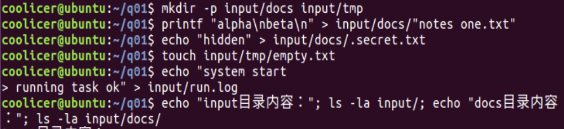
\includegraphics[width=1\textwidth]{1.1.png} 
\end{figure}

步骤2:查看路径与列表
\\echo "q01绝对路径：" \&\& pwd   ---------pwd:输出当前绝对路径 
 \\输出：/home/coolicer/q01
\\ls -la input/     ----------------------------l长格式，-a显示隐藏文件
 \\含隐藏文件，确认 docs、tmp、run.log

 步骤3：复制txt文件（保留结构，处理空格）
 \\STUID="2502000718"-------------定义学号变量，后续\$STUID调用
\\mkdir -p work/\$STUID ------------创建目标目录
\\rsync -avm --include='*.txt' --include='*/' --exclude='*' input/ work/\$STUID/ 
\\--include='*.txt'：包含全部 txt 文件（匹配含空格的 notes one.txt）
\\--include='*/'：包含所有目录（确保相对路径结构）
\\--exclude='*'：排除所有其他内容（如 run.log 非 txt，被排除）
\\rsync用于复制，work/\$STUID/为目标路径

\begin{figure}[H]
    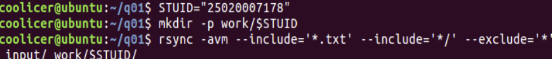
\includegraphics[width=1\textwidth]{1.2.png} 
\end{figure}
步骤4：权限设置于清单生成
\begin{lstlisting}[language=bash, basicstyle=\ttfamily\small]
find work/$STUID -type d -exec chmod 750 {} 
find work/$STUID -type f -exec chmod 640 {} +
cd work/$STUID && find . -type f -exec stat -c '%n %s' {} \; > ../../inventory.txt
cat ../../inventory.txt 
\end{lstlisting}
% find work/$STUID：从 work/你的学号目录开始递归查找。
% -type d：筛选条件，仅匹配目录（directory）
% -exec ... {} +：对查找到的结果执行后续命令。
% {} 是占位符，代表查到的路径；+ 表示将所有结果合并一次性执行
% chmod 750：修改权限
% -type f：仅匹配普通文件（file）
% -exec stat -c "%n %s" {} \;：
% stat：查看文件详细信息。
% -c "%n %s"：自定义输出格式，%n 输出文件名（相对路径），%s 输出字节数，中间空格分隔。
% > ../../inventory.txt：重定向输出。
% 当前在 work/学号/，../.. 即回到 q01/，将结果写入 inventory.txt

4. 实验结果验证\\
目录结构：work/2502000718/input/{docs,tmp} 下仅含 .txt 文件，含空格文件 notes one.txt 完整复制。
\\权限：目录 750（drwxr-x---），文件 640（-rw-r-----）。
\\inventory.txt 内容：
\\纯文本
\\./docs/.secret.txt 7
\\./docs/notes one.txt 11
\\./tmp/empty.txt 0
\\符合“相对路径+字节数”的要求





\newpage
\subsection{实验2：随机访问日志统计}


\subsubsection{操作过程与命令解析}

步骤1. 目录创建与数据准备\\
在 q02 目录下，通过 cat << EOF 创建 access.csv，
包含 1 行表头与 8 行访问日志。为后续统计提供原始数据。
\begin{figure}[H]
    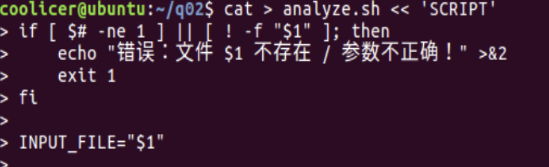
\includegraphics[width=1\textwidth]{2.1.png}
\end{figure}

步骤2. 编写analyze.sh与参数校验\\
通过 \texttt{cat > analyze.sh << 'SCRIPT'} 写入脚本，核心逻辑如下：
\begin{itemize}
    \item \textbf{参数校验}：\texttt{if [ \$\# -ne 1 ] || [ ! -f "\$1" ]} 判断参数数量是否为 1 且文件是否存在；若异常则 \texttt{echo "错误..." >\&2}（重定向到标准错误stderr），并执行 \texttt{exit 1}返回非零退出码。
    \item \textbf{变量赋值}：\texttt{INPUT\_FILE="\$1"} 记录文件路径。\\SCRIPT:结束脚本写入
\end{itemize}
步骤3. HTTP 5xx统计
\begin{itemize}
    \item \textbf{5xx 统计}：\texttt{tail -n +2} 跳过表头 $\rightarrow$ \texttt{awk -F',' '\$4 >= 500 \{print \$3\}'} 以逗号为分隔符，筛选第4列（status）≥500（5xx），输出第3列（path） $\rightarrow$ \texttt{sort | uniq -c} 计数 $\rightarrow$ \texttt{sort -k1nr -k2d} 按次数降序、路径字典序排 $\rightarrow$ \texttt{head -n2} 取前 2 $\rightarrow$ \texttt{awk '\{printf "\%s : \%d次\textbackslash n", \$2, \$1\}'} 格式化输出。
\end{itemize}
\begin{figure}[H]
    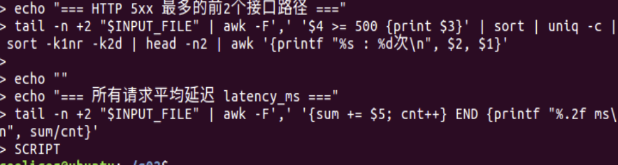
\includegraphics[width=1\textwidth]{2.2.png}
\end{figure}
步骤4.平均延迟时间计算
\begin{itemize}
    \item \textbf{平均延迟}：\texttt{tail -n +2} 跳过表头 $\rightarrow$ \texttt{awk -F',' '\{sum += \$5; cnt++\} END \{printf "\%.2f ms\textbackslash n", sum/cnt\}'} 累加第 5 列并求均值，保留两位。\%.2f：强制保留两位小数
    \item tail:默认用于查看文件末尾内容
    \item "\$INPUT\_FILE":传入的CSV文件路径。加双引号可避免路径含空格时出错
\end{itemize}
写入后执行 \texttt{chmod +x analyze.sh} 赋予可执行权限。
\begin{figure}[H]
    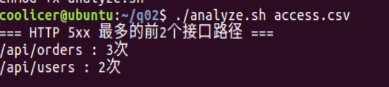
\includegraphics[width=1\textwidth]{2.3.png}
\end{figure}
\subsubsection{运行测试与结果验证}
\begin{itemize}
    \item \textbf{正常执行}：\texttt{./analyze.sh access.csv} 输出：
    \begin{verbatim}
=== HTTP 5xx 最多的前2个接口路径 ===
/api/orders : 3次
/api/users : 2次
=== 所有请求平均延迟 latency_ms ===
193.75 ms
    \end{verbatim}
    结果符合数据特征（orders 出现 3 次 5xx，users 2 次；总延迟 1550ms/8条=193.75ms）。
    \item \textbf{异常执行}：\texttt{./analyze.sh 不存在的文件.csv} 输出 \texttt{错误：文件 不存在的文件.csv 不存在 / 参数不正确！} 到 \texttt{stderr}，随后 \texttt{echo "脚本退出码：\$?"} 显示 \texttt{1}，符合非零退出要求。
\end{itemize}
\subsection{实验3：制造、解决并解释一次合并冲突}

\subsubsection{操作过程与命令解析}
\begin{itemize}
    \item \textbf{初始化与配置}：执行 \texttt{git init} 初始化仓库。通过 \texttt{git config} 设置用户身份。使用 \texttt{echo} 重定向写入 \texttt{config.txt} 并 \texttt{git commit} 完成初始提交。执行 \texttt{git branch -M main} 设定主分支。
\begin{figure}[H]
    
 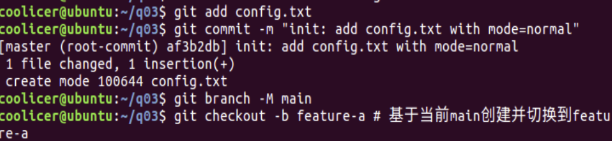
\includegraphics[width=1\textwidth]{3.1.png} 
\end{figure}
\vspace{-0.5cm} % 向下压缩空白
    \item \textbf{分支开发与冲突制造}：使用 \texttt{git checkout -b feature-a} 创建特性分支并修改为 \texttt{mode=safe} 提交；切回 \texttt{main} 后，基于初始状态创建 \texttt{feature-b} 并修改为 \texttt{mode=fast} 提交。两分支对同一文件行做了不同修改。
    \begin{figure}[H]
    
 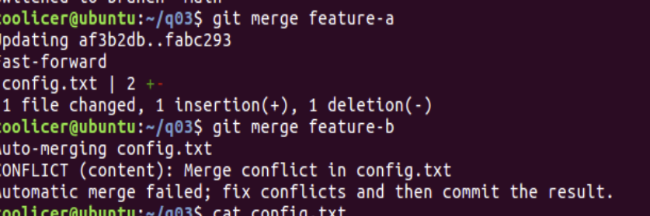
\includegraphics[width=1\textwidth]{3.2.png} 
\end{figure}
    \item \textbf{合并与冲突解决}：切回 \texttt{main}，\texttt{git merge feature-a} 提示 \texttt{Fast-forward} 成功。合并 \texttt{feature-b} 时提示 \texttt{CONFLICT (content)}。通过 \texttt{cat} 查看冲突标记（\texttt{<<<<<<< HEAD} 等）。使用 \texttt{cat > config.txt << 'EOF'} 覆盖写入最终内容（保留 \texttt{safe} 加 \texttt{note=reviewed}）。执行 \texttt{git add} 标记已解决，并提交合并信息。
\end{itemize}
\begin{figure}[H]
    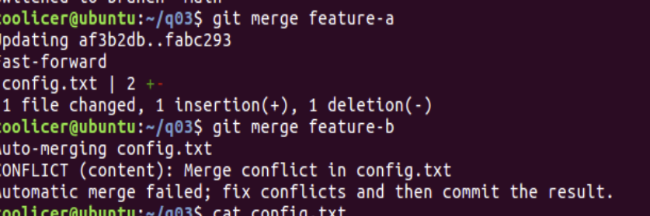
\includegraphics[width=1\textwidth]{3.2.png}
    \caption{Git 合并历史拓扑图验证}
\end{figure}
\subsubsection{运行测试与结果验证}
\begin{itemize}
    \item \textbf{状态与历史验证}：执行 \texttt{git status} 确认工作区干净（\texttt{working directory clean}）。
    \item \textbf{拓扑图验证}：执行 \texttt{git log --all --graph --decorate --oneline}，终端输出图形化历史，确认 \texttt{feature-a} 和 \texttt{feature-b} 的节点已合并入 \texttt{main}，符合题目要求的分支拓扑结构。
\end{itemize}
\begin{figure}[H]
    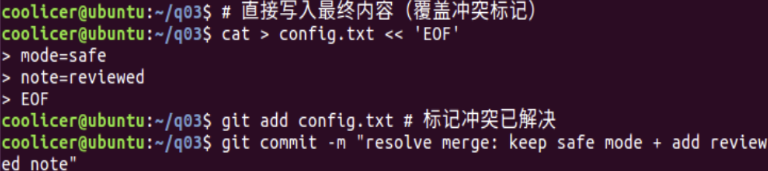
\includegraphics[width=1\textwidth]{3.3.png}
    \caption{Git 结果验证}
\end{figure}




\newpage
\subsection{实验4：修复并构建一页技术说明}

\subsubsection{操作过程与命令解析}
\begin{itemize}
    \item \textbf{目录创建与文档编写}：执行 \texttt{mkdir -p q04} 创建实验目录并进入。使用 \texttt{nano report.tex} 创建并编辑 LaTeX 源码文件，补全文档类、宏包、公式、表格和交叉引用代码。
    \begin{figure}[H]
        \centering
        
\includegraphics[width=0.8\textwidth]{4.1.png} % 替换为实际截图
        \caption{创建 q04 目录并编辑 report.tex}
    \end{figure}
    \vspace{-0.5cm}

    \item \textbf{文档结构与公式}：使用 \texttt{\textbackslash documentclass\{article\}} 初始化文档，引入 \texttt{amsmath} 宏包支持数学公式与 \texttt{\textbackslash eqref} 引用。
\\引入公式：\verb|\begin{equation}|
\\结束公式：\verb|\end{equation}|
    \item \textbf{表格与标签}：使用 \texttt{table} 浮动环境和 \texttt{tabular} 环境绘制 2 行 2 列表格，通过 \texttt{\textbackslash caption\{系统性能参数\}} 添加标题，并在其后紧跟 \texttt{\textbackslash label\{tab:perf\}}。注意：\texttt{label} 必须放在 \texttt{caption} 之后。

    \item \textbf{交叉引用}：
    \\ \verb|\eqref{eq:throughput}| 引用公式编号并自动加括号，输出为 “(1)”；
    \\ \verb|\ref{tab:env}| 输出表格编号 “1”       
    \item \textbf{命令行构建}：在终端执行 \texttt{latexmk -pdf -halt-on-error report.tex}（或 \texttt{tectonic report.tex}）编译生成 PDF。
\end{itemize}

\begin{figure}[H]
    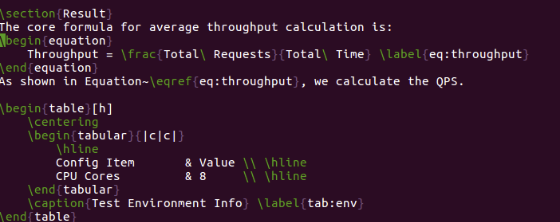
\includegraphics[width=1\textwidth]{4.2.png} 
    \caption{LaTeX 编译生成 PDF 部分代码展示}
\end{figure}

\subsubsection{运行测试与结果验证}

\begin{itemize}
    \item \textbf{PDF 生成验证}：编译成功后当前目录会出现 \texttt{report.pdf}，使用 \texttt{evince report.pdf \&} 打开查看。

    \item \textbf{交叉引用验证}：由于 LaTeX 需要多遍编译，首次编译引用处可能显示 \texttt{??}。连续编译两次后，确认公式引用显示为 \texttt{(1)}，表格引用显示为 \texttt{1}，不再出现 \texttt{??}。
\end{itemize}

\begin{figure}[H]
    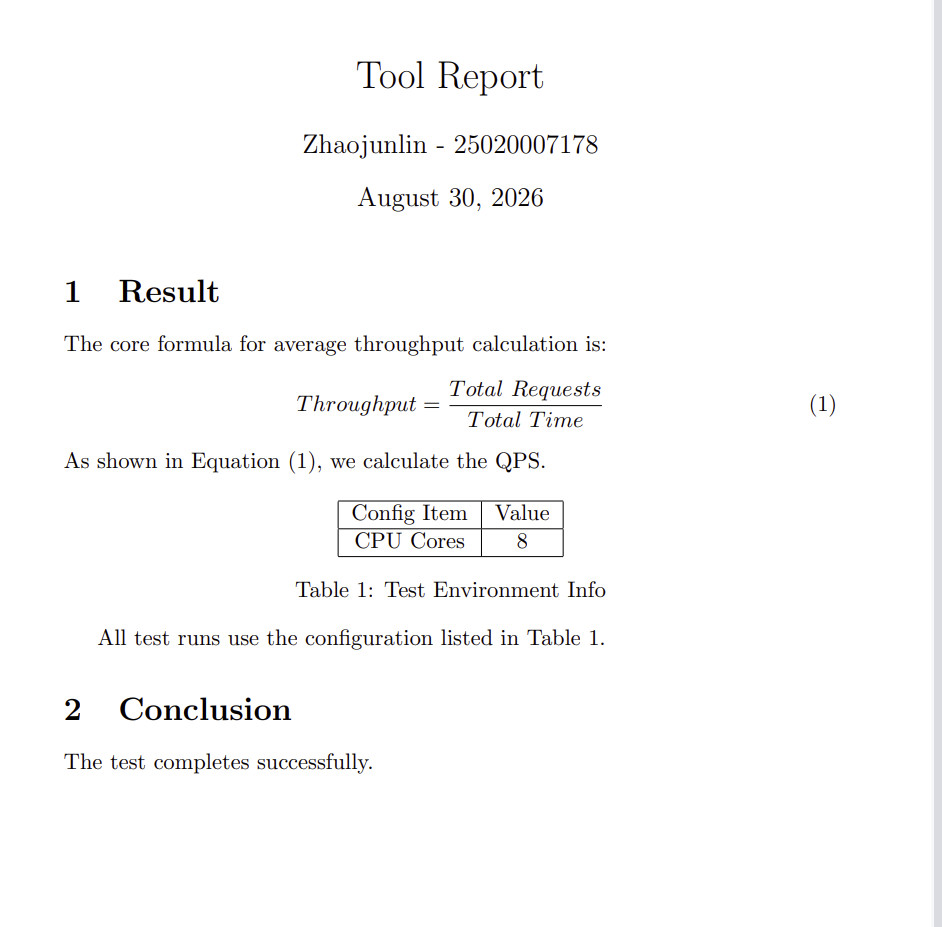
\includegraphics[width=1\textwidth]{4.3.png} 
    \caption{PDF 预览与交叉引用结果验证}
\end{figure}

\newpage

\section{练习：Shell入门}
\subsection{ls的作用}
ls -l 的作用是以长格式（long format）显示文件详细信息。
与直接输入 ls 仅显示文件名不同，ls -l 会显示文件的权限、硬链接数、
所有者、所属组、文件大小、最后修改时间和文件名。
\begin{figure}[H]
 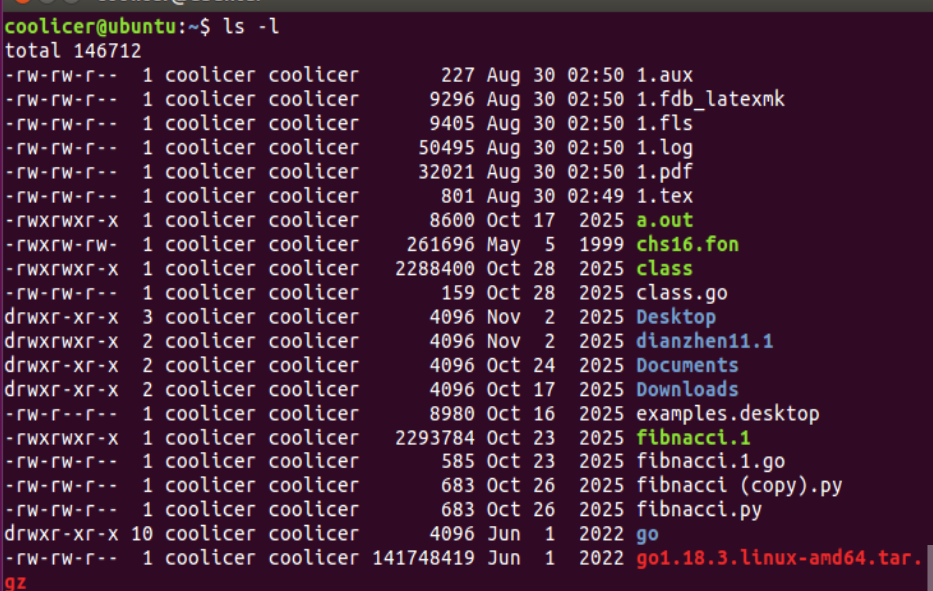
\includegraphics[width=1\textwidth]{10.1.png} 
\end{figure}

\begin{table}[h]
\centering
\small % 稍微缩小表格字体
\begin{tabular}{|c|c|p{6cm}|}
\hline
位次 & 常见取值 & 含义 \\
\hline
1 & \texttt{d/-/l/b/c/a/p} & 文件类型 \\
\hline
2 & \texttt{r/-} & 所有者读权限 \\
\hline
3 & \texttt{w/-} & 所有者写权限 \\
\hline
4 & \texttt{x/-/s} & 所有者执行权限（\texttt{s}=setuid） \\
\hline
5 & \texttt{r/-} & 所属组读权限 \\
\hline
6 & \texttt{w/-} & 所属组写权限 \\
\hline
7 & \texttt{x/-/s} & 所属组执行权限（\texttt{s}=setgid） \\
\hline
8 & \texttt{r/-} & 其他用户读权限 \\
\hline
9 & \texttt{w/-} & 其他用户写权限 \\
\hline
10 & \texttt{x/-/t} & 其他用户执行权限（\texttt{t}=粘滞位） \\
\hline
\end{tabular}
\caption{\texttt{ls -l} 输出前 10 个字符的含义}
\label{tab:ls-l}
\end{table}

\subsection{三种引号的区别与特殊字符输出}
\begin{itemize}
    \item \textbf{单引号''}：强引用，内部所有字符（包括 \$、反引号、转义符）都被原样保留，不解析。
    \item \textbf{双引号""}：弱引用，允许解析 \verb|$|（变量）、反引号（命令替换）、\verb|`|（转义）和 \verb|!|（历史扩展）。
    \item \textbf{ANSI-C 引号} \verb|$' '|：支持解析反斜杠转义序列（如 \verb|\n| 换行、\verb|\a| 响铃）。
\end{itemize}
\begin{figure}[H]
 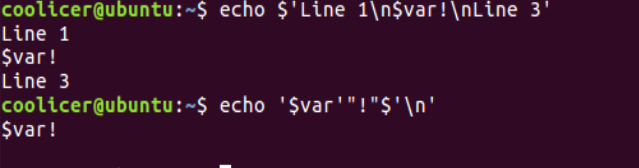
\includegraphics[width=1\textwidth]{10.2.png} 
\end{figure}

\subsection{为什么cd必须是Shell内建命令}
原理：Linux/Unix 的进程模型规定，每个进程只能修改自己的当前工作目录（cwd），
子进程无法修改父进程的环境。如果 cd 是独立程序，Shell 会 fork 出一个子进程去执行 cd，
子进程目录改了但随即退出，父进程（你的交互式 Shell）目录纹丝不动。因此 cd 必须是内建命令，
直接在 Shell 进程内调用 chdir() 系统调用。\\
验证cd是内建命令：
\begin{figure}[H]
 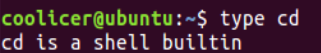
\includegraphics[width=1\textwidth]{10.3.png} 
\end{figure}

\subsection{脚本赋权与执行}
原理：Linux 下直接运行 ./script.sh 需要该文件具备可执行权限（x）。
新建的脚本默认没有执行权限，需要通过 chmod +x 添加
\begin{figure}[H]
 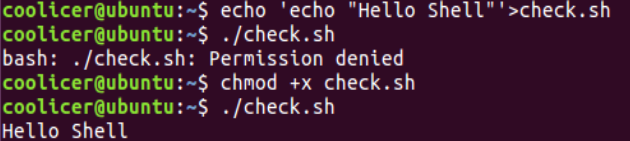
\includegraphics[width=1\textwidth]{10.4.png} 
\end{figure}

\subsection{命令替换与日期备份}
原理：\$(command) 会将括号内命令的执行结果替换到当前位置。
结合 date 命令格式化输出，可动态生成带日期的文件名。
\begin{figure}[H]
 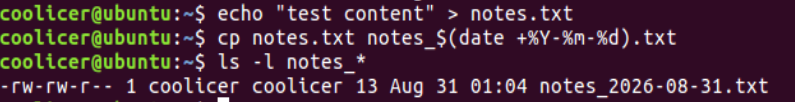
\includegraphics[width=1\textwidth]{10.5.png} 
\end{figure}

\subsection{使用awk按列过滤与交换字段}
原理：awk 默认按空格/制表符分列（\$1, \$2, \$3...）。
可以通过条件判断过滤行，并重新赋值列内容后打印。
\begin{figure}[H]
 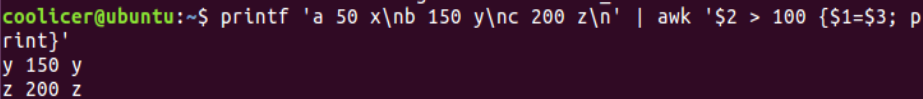
\includegraphics[width=1\textwidth]{10.6.png} 
\end{figure}
\newpage

\subsection{克隆本课程网站的仓库}
git clone命令来克隆仓库，并转到克隆后的仓库目录下
\begin{figure}[H]
 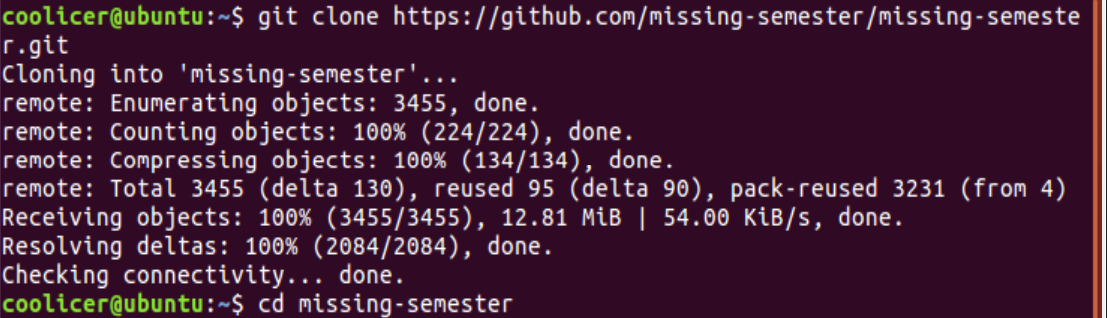
\includegraphics[width=1\textwidth]{10.7.1.png} 
\end{figure}

\subsubsection{可视化版本历史为图}
git log命令查看版本历史，--all参数来显示所有分支的提交情况，
\\--graph将路径画成图形
\begin{figure}[H]
 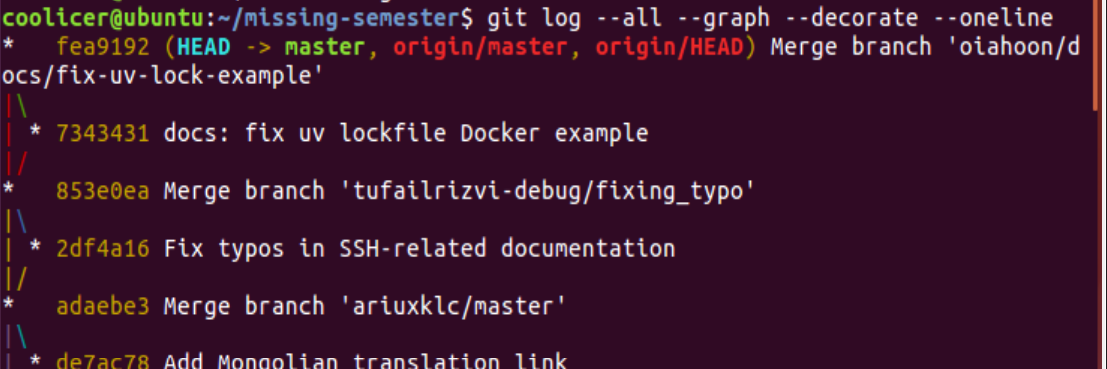
\includegraphics[width=1\textwidth]{10.7.2.png} 
\end{figure}

\subsubsection{查看最后修改README.md的人}
git log查看仓库里的提交历史记录\\
README.md：只看跟README.md这个文件有关的提交记录；\\
-1：只看其中最近的一条记录
\begin{figure}[H]
 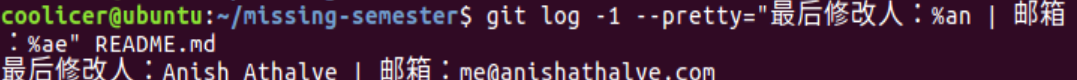
\includegraphics[width=1\textwidth]{10.7.4.png} 
\end{figure}

\subsection{配置Git别名}
目标：让 git graph
等价于长命令 git log --all --graph --decorate --oneline
\begin{figure}[H]
 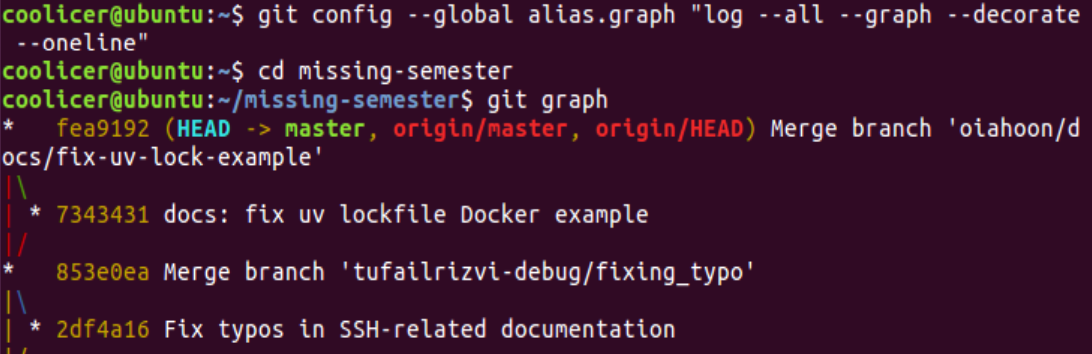
\includegraphics[width=1\textwidth]{10.8.png} 
\end{figure}

\subsection{配置全局.gitignore}
目标：所有仓库自动忽略.DS\_Store/编辑器缓存这类不需要提交的文件
\begin{figure}[H]

 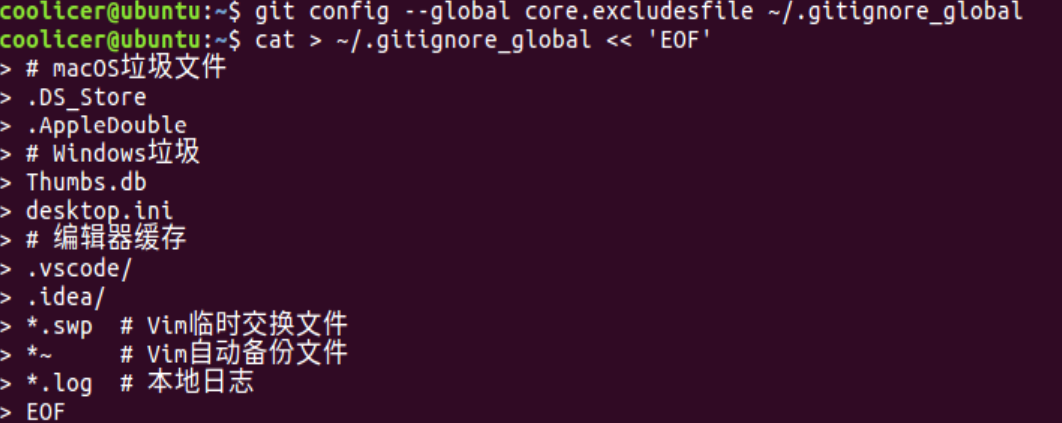
\includegraphics[width=1\textwidth]{10.9.png} 
\end{figure}

\subsection{模拟合并冲突+解决}
目标：体验两人改同一行代码的冲突处理流程\\
git init：把当前文件夹初始化成一个空的 Git 仓库(开始用git管理代码)\\
cat > recipe.txt << 'EOF' ... EOF：新建一个叫 recipe.txt 的文件，
并往里面写入食谱内容（直到遇到 EOF 结束）\\
\begin{figure}[H]
 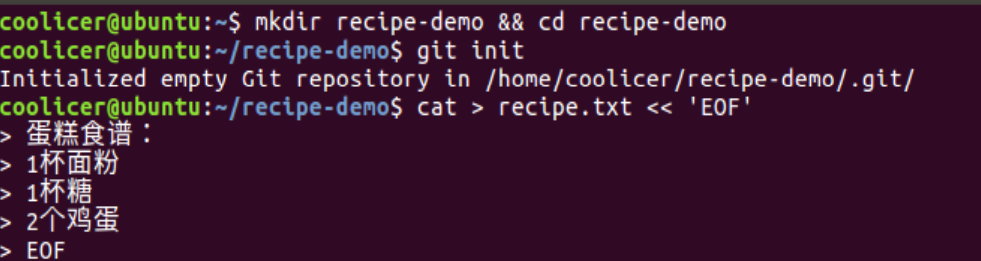
\includegraphics[width=1\textwidth]{10.10.1.png} 
\end{figure}
git add . \&\& git commit -m "初始食谱"：把刚才写好的文件交给 Git 暂存，
然后正式提交到仓库，提交说明叫“初始食谱”。\\
git branch sweet创建分支，git chekout sweet切到sweet分支

\begin{figure}[H]
    
 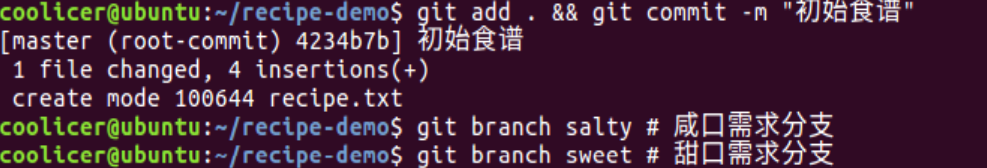
\includegraphics[width=1\textwidth]{10.10.2.png} 
\end{figure}
sed -i 's/1杯糖/2杯糖/' recipe.txt：把文件里的“1杯糖”改成“2杯糖”。

\begin{figure}[H]
    
 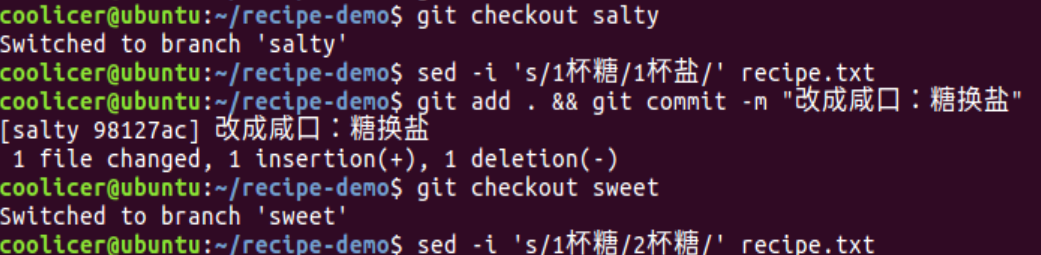
\includegraphics[width=1\textwidth]{10.10.3.png} 
\end{figure}
git add . \&\& git commit -m "改成超甜：糖加量为2杯"：修改保存并提交
\begin{figure}[H]
    
 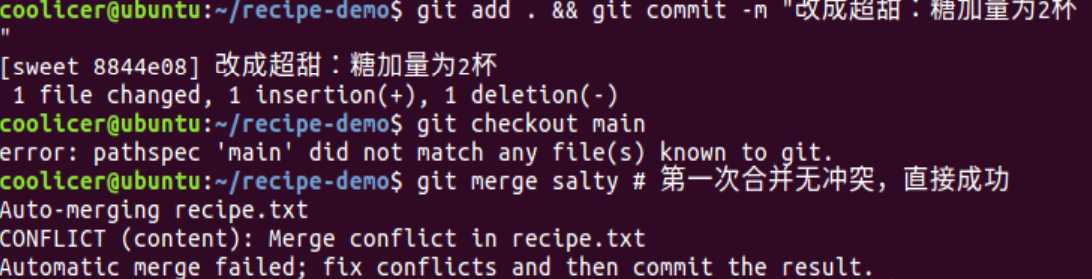
\includegraphics[width=1\textwidth]{10.10.4.png} 
\end{figure}
手动重新编辑文件，删除Git生成的冲突标记并提交

\begin{figure}[H]
    
 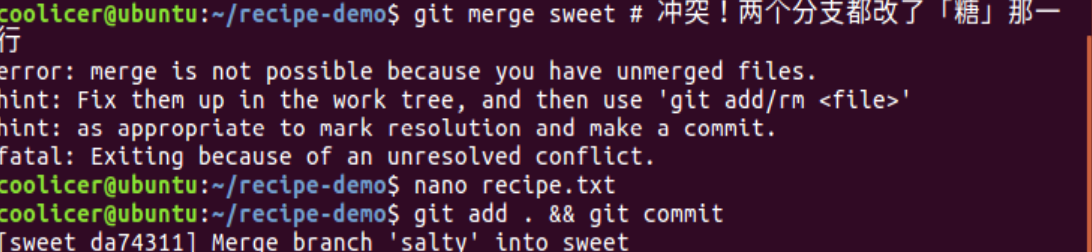
\includegraphics[width=1\textwidth]{10.10.5.png} 
\end{figure}
以树状图查看刚才的完整历史记录

\begin{figure}[H]
    
 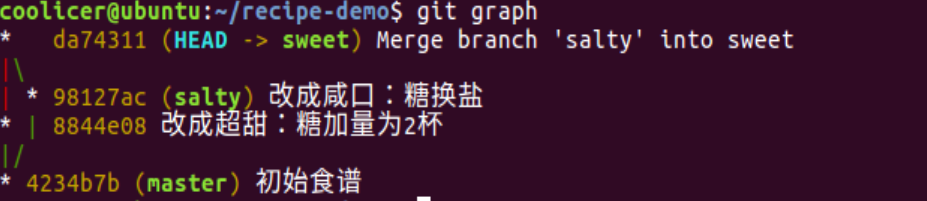
\includegraphics[width=1\textwidth]{10.10.6.png} 
\end{figure}


\newpage
\section{实验心得}
通过本次实验，我学会了基本的使用git来进行版本控制的操作方法，
以及对如何运用latex进行文档的编辑与排版，感受到了latex编辑与word编辑的
不同和它在模版使用方面的便利。
\end{document}
